% Preamble
\documentclass[11pt]{article}

% Packages
\usepackage{amsmath}
\usepackage[a4paper, margin=0.5in]{geometry}
\usepackage{graphicx} % daj an 1in jak chcesz normalniejszy margines, ale kod mi się w linii nie mieści :P
\usepackage[utf8]{inputenc}
\usepackage[T1]{fontenc}
\usepackage[polish]{babel}
\usepackage{float}
\usepackage{hyperref}
\usepackage{cleveref}

\title{Zadanie 1. Heurystyki konstrukcyjne}
\author{Oskar Kiliańczyk 151863 \& Wojciech Kot 151876}
\date{}

% Document
\begin{document}

\maketitle
\newpage

\section{Opis zadania}\label{sec:opis-zadania}

Podczas zajęć rozważamy zmodyfikowany problem komiwojażera.
Początkowo, obliczamy macierz odległości pomiędzy danymi miastami.
Obliczona macierz odległości między wierzchołkami grafu będzie podstawą dla każdego algorytmu,
a celem jest wyznaczenie dwóch rozłącznych zamkniętych ścieżek (cykli), z których każda zawiera 50\% wierzchołków.
Jeśli liczba wierzchołków jest nieparzysta, jedna ścieżka zawiera jeden wierzchołek więcej.
Kryterium optymalizacji jest minimalizacja łącznej długości obu cykli.

Rozważane instancje problemu pochodzą z biblioteki TSPLib, a są to kroA200 oraz kroB200.
Są to instancje dwuwymiarowe euklidesowe, w których każdemu wierzchołkowi przypisane są współrzędne na płaszczyźnie.
Odległość między wierzchołkami liczona jest jako odległość euklidesowa, zaokrąglana do najbliższej liczby całkowitej.
W implementacji algorytmów wykorzystywana będzie wyłącznie macierz odległości, co zapewni możliwość zastosowania kodu do innych instancji problemu.

\section{Zaimplementowane algorytmy}\label{sec:zaimplementowane-algorytmy}

\subsection{Algorytm zachłanny - metoda najbliższego sąsiada}\label{subsec:algorytm-zachanny---metoda-najblizszego-sasiada}

Algorytm ten wykorzystuje funkcję znajdującą najbliższego sąsiada dla danego wierzchołka (miasta).
Działa ona w następujący sposób:
\begin{enumerate}
\item Dla każdego miasta, sprawdza czy zostało już odwiedzone
\item Jeśli nie, to sprawdza czy dystans jest mniejszy od dystansu z danego miasta do obecnie zapamiętanego jako najbliższe
\item Jeśli jest bliższe niż obecnie pamiętane jako najbliższe, zapamiętuje je jako najbliższe
\item Jeśli nie ma żadnego miasta obecnie pamiętanego jako najbliższe, przypisuje to miasto
\end{enumerate}

Główny algorytm natomiast, wygląda następująco:

\begin{enumerate}
    \item Przydziela wierzchołki startowe do cykli pierwszego i drugiego.
    \item Tworzy tablicę indeksów miast, zaznaczając wszystkie poza startowymi jako nieodwiedzone.
    \item Dopóki istnieją jakieś nieodwiedzone miasta, powtarza następujące kroki:
    \begin{itemize}
        \item Znajduje najbliższego nieodwiedzonego sąsiada do ostatniego wierzchołka cyklu 1.
        \item Dodaje go do cyklu 1 oraz zapisuje w tablicy jako odwiedzony.
        \item Znajduje najbliższego nieodwiedzonego sąsiada do ostatniego wierzchołka cyklu 2.
        \item Dodaje go do cyklu 2 oraz zapisuje w tablicy jako odwiedzony.
    \end{itemize}
    \item Kiedy już nie ma żadnych nieodwiedzonych miast, dopisuje na koniec cykli ich wierzchołki startowe.
    \item Zwraca oba cykle jako znalezione ścieżki.
\end{enumerate}


\subsection{Algorytm zachłanny - metoda rozbudowy cyklu}\label{subsec:algorytm-zachanny---metoda-rozbudowy-cyklu}

Algorytm ten korzysta z funkcji znajdywania najlepszego wstawienia, a działa ona w następujący sposób:

\begin{enumerate}
    \item Przyjmuje jako argumenty:
    \begin{itemize}
        \item obecny cykl,
        \item macierz dystansów,
        \item tablicę indeksów odwiedzonych miast.
    \end{itemize}
    \item Tworzy listę możliwości (nieodwiedzonych wierzchołków).
    \item Ustawia najtańszy koszt na maksymalnie dużą wartość.
    \item Dla każdej możliwości z listy możliwości:
    \begin{enumerate}
        \item Dla każdego możliwego wstawienia w cykl:
        \begin{itemize}
            \item Oblicza wzrost dystansu, jaki spowoduje wstawienie (a więc przy wstawianiu między \(a\) i \(b\) wierzchołka \(c\), oblicza dystans \(|ac| + |bc| - |ab|\)).
            \item Zapisuje najmniejszy znaleziony wzrost dystansu oraz miejsce jego wstawienia.
        \end{itemize}
        \item Jeśli koszt wstawienia obecnie znalezionego wierzchołka jest mniejszy niż obecnie pamiętany najtańszy koszt wstawienia:
        \begin{itemize}
            \item Zapisuje ten koszt jako obecnie najtańszy.
            \item Zapisuje wierzchołek oraz miejsce jego wstawienia.
        \end{itemize}
    \end{enumerate}
    \item Po przejrzeniu wszystkich możliwości zwraca parę \(\langle\)wierzchołek, miejsce wstawienia\(\rangle\).
\end{enumerate}

Sam algorytm:
\begin{enumerate}
    \item Dwukrotnie przydziela wierzchołki startowe do cykli pierwszego i drugiego jako początek i koniec cyklu.
    \item Tworzy tablicę indeksów miast, zaznaczając wszystkie poza startowymi jako nieodwiedzone.
    \item Dopóki istnieją jakieś nieodwiedzone miasta, powtarza następujące kroki:
    \begin{enumerate}
        \item Znajduje najtańsze wstawienie, czyli parę \(\langle\)wierzchołek, miejsce w cyklu\(\rangle\) dla cyklu 1.
        \item Wstawia w odpowiednie miejsce cyklu 1 znaleziony wierzchołek.
        \item Zapisuje wierzchołek jako już odwiedzony.
        \item Znajduje najtańsze wstawienie dla cyklu 2.
        \item Jeśli ono nie istnieje (np. bo ostatni wierzchołek został już wstawiony), to kończy pętlę.
        \item Wstawia w odpowiednie miejsce cyklu 2 znaleziony wierzchołek.
        \item Zapisuje wierzchołek jako już odwiedzony.
    \end{enumerate}
    \item Kiedy już nie ma żadnych nieodwiedzonych miast, zwraca oba cykle jako znalezione ścieżki.
\end{enumerate}


\subsection{Algorytm z żalem - metoda rozbudowy cyklu}\label{subsec:algorytm-z-zalem---metoda-rozbudowy-cyklu}

\begin{enumerate}
    \item Dwukrotnie przydziela wierzchołki startowe do cykli pierwszego i drugiego jako początek i koniec cyklu.
    \item Tworzy tablicę indeksów miast, zaznaczając wszystkie poza startowymi jako nieodwiedzone.
    \item Dopóki istnieją jakieś nieodwiedzone miasta, powtarza następujące kroki:
    \begin{enumerate}
        \item Dla każdego cyklu:
        \begin{enumerate}
            \item Oblicz koszt rozbudowy cyklu o każde możliwe nieodwiedzone dotąd miasto dla każdego możliwego punktu rozbudowy cyklu.
            \item Posortuj listę kosztów (rosnąco).
            \item Oblicz dwużal jako różnicę pomiędzy drugim najlepszym a najlepszym wynikiem z listy kosztów.
            \item Jeżeli wyliczony żal jest większy niż dla jakiegokolwiek innego wstawienia miasta, to uznaj go za najlepszy.
        \end{enumerate}
        \item Rozszerz cykl w miejscu wskazanym dla najlepszego wyliczonego dwużalu.
        \item Zapisz wierzchołek jako już odwiedzony.
    \end{enumerate}
    \item Kiedy już nie ma żadnych nieodwiedzonych miast, zwraca oba cykle jako znalezione ścieżki.
\end{enumerate}


\subsection{Algorytm z żalem - metoda rozbudowy cyklu z żalem ważonym}\label{subsec:algorytm-z-zalem---metoda-rozbudowy-cyklu-z-zalem-wazonym}

\begin{enumerate}
    \item Dwukrotnie przydziela wierzchołki startowe do cykli pierwszego i drugiego jako początek i koniec cyklu.
    \item Tworzy tablicę indeksów miast, zaznaczając wszystkie poza startowymi jako nieodwiedzone.
    \item Dopóki istnieją jakieś nieodwiedzone miasta, powtarza następujące kroki:
    \begin{enumerate}
        \item Dla każdego cyklu:
        \begin{enumerate}
            \item Oblicz koszt rozbudowy cyklu o każde możliwe nieodwiedzone dotąd miasto dla każdego możliwego punktu rozbudowy cyklu.
            \item Posortuj listę kosztów (rosnąco).
            \item Oblicz dwużal ważony jako różnicę pomiędzy drugim najlepszym a najlepszym wynikiem z listy kosztów z odpowiednimi wagami (domyślnie $waga_2 = (-1) \cdot waga_1$).
            \item Jeżeli wyliczony żal jest większy niż dla jakiegokolwiek innego wstawienia miasta, to uznaj go za najlepszy.
        \end{enumerate}
        \item Rozszerz cykl w miejscu wskazanym dla najlepszego wyliczonego dwużalu.
        \item Zapisz wierzchołek jako już odwiedzony.
    \end{enumerate}
    \item Kiedy już nie ma żadnych nieodwiedzonych miast, zwraca oba cykle jako znalezione ścieżki.
\end{enumerate}

\subsection{Nasz własny algorytm}\label{subsec:nasz-wasny-algorytm}

Po zobaczeniu wyników dla pierwszych czterech opisanych tu algorytmów zdecydowaliśmy się na napisanie jeszcze jednego, własnego algorytmu.
Głównym powodem było nasze ogromne niezadowolenie ze skuteczności podejścia korzystającego z dwużalu, oraz to jaki potencjał w tym podejściu zauważyliśmy.
Jak da się zauważyć w tabeli~\ref{tab:wyniki-eksperymentu} zamieszczonej w~\ref{sec:wyniki-eksperymenty-obliczeniowego} algorytmy oparte na dwużalu nie osiągnęły zadowalających nas wyników,
wobec czego wyciągnęliśmy wnioski opsisane w~\ref{sec:wnioski} i zdecydowaliśmy się skorzystać z dwużalu dzieląc wcześniej zbiór wierzchołków na dwa równe podzbiory,
a następnie rozwiązanie standardowego problemu komiwojażera na każdym z podzbiorów.
Trzymając się tematu zajęć podział na podzbiory został wykonany podejściem zachłannym:

\begin{enumerate}
    \item Utworzenie listy pozostałych wierzchołków (wszystkie możliwe, poza startowymi)
    \item Utworzenie dwóch list zawierających odpowiednio dystanse każdego wierzchołka do pierwszego i do drugiego wierzchołka startowego
    \item Sortowanie utworzonych uprzednio list dystansów wierzchołków
    \item Aż do przydzielenia wszystkich wierzchołków z listy pozostałych wierzchołków wykonuje:
    \item Zmianę decyzji do którego zestawu wierzchołków obecnie będzie przydzielać wierzchołek (aby robić to naprzemiennie)
    \item Wyszukuje pierwszy wierzchołek na liście dystansów który nie został jeszcze przydzielony do żadnego zestawu i przydziela go tam
\end{enumerate}

W skutek zastosowania takiego przydziału uzyskujemy dwa równo-liczne zbiory, oraz zapewniamy że gdyby ilość badanych wierzchołków była nieparzysta, to zbiory będą różnić się długością najwyżej o 1.

Następnie wykorzystujemy tradycyjny algorytm rozbudowy cyklu w oparciu o dwużal, osobno na obu listach. Wygląda on następująco:

\begin{enumerate}
    \item Algorytm zaczyna od ścieżki zawierającej wierzchołek startowy podwójnie
    \item Dopóki w ścieżce nie znajdują sie wszystkie wierzchołki z zadanego mu zestawu powtarza:
    \item Dla każdego nieodwiedzonego wierzchołka oblicza koszty jego wstawienia
    \item Następnie oblicza żal (dwużal) dla danego wierzchołka
    \item Rozbudowuje cykl o wierzchołek z największym obliczonym żalem i zaznacza go jako odwiedzonego
    \item Zwraca ścieżkę
\end{enumerate}

Używając takiej funkcji osobno na obu zbiorach wierzchołków uzyskujemy dwie ścieżki i zwracamy do programu głównego.


\section{Wyniki eksperymentu obliczeniowego}\label{sec:wyniki-eksperymenty-obliczeniowego}

\subsection{Algorytm zachłanny - metoda najbliższego sąsiada}\label{subsec:algorytm-zachanny---metoda-najblizszego-sasiada2}
Graficzną reprezentację wyników dla algorytmu zachłannego metodą najbliższego sąsiada przestawiono na~\ref{fig:Greedy-nearest-kroA} oraz~\ref{fig:Greedy-nearest-kroB}.

\begin{figure}[H]
    \centering
    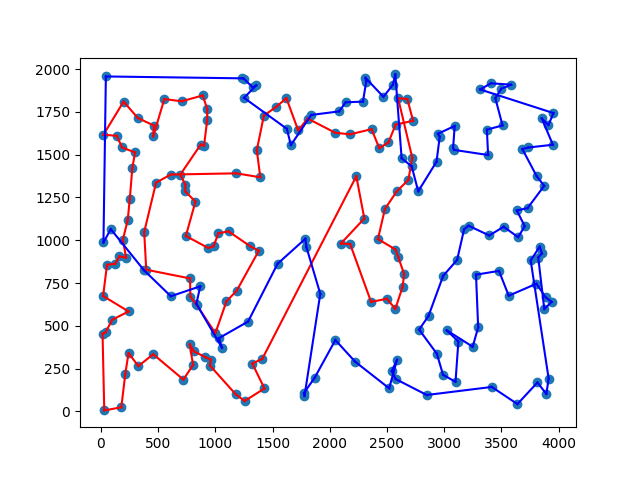
\includegraphics{best_paths/greedy_nearest_neighbor_kroA200.tsp.png}
    \caption{Instancja kroA200}
    \label{fig:Greedy-nearest-kroA}
\end{figure}
\begin{figure}[H]
    \centering
    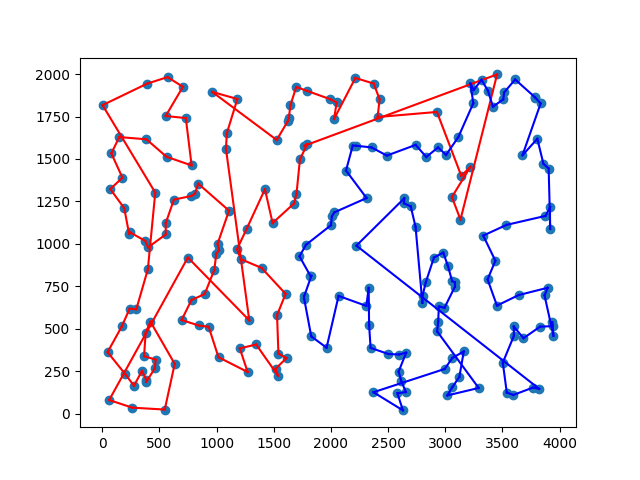
\includegraphics{best_paths/greedy_nearest_neighbor_kroB200.tsp.png}
    \caption{Instancja kroB200}
    \label{fig:Greedy-nearest-kroB}
\end{figure}

\subsection{Algorytm zachłanny - metoda rozbudowy cyklu}\label{subsec:algorytm-zachanny---metoda-rozbudowy-cyklu2}
Graficzną reprezentację wyników dla algorytmu zachłannego metodą rozbudowy cyklu przestawiono na~\ref{fig:Greedy-cycle-kroA} oraz~\ref{fig:Greedy-cycle-kroB}.

\begin{figure}[H]
    \centering
    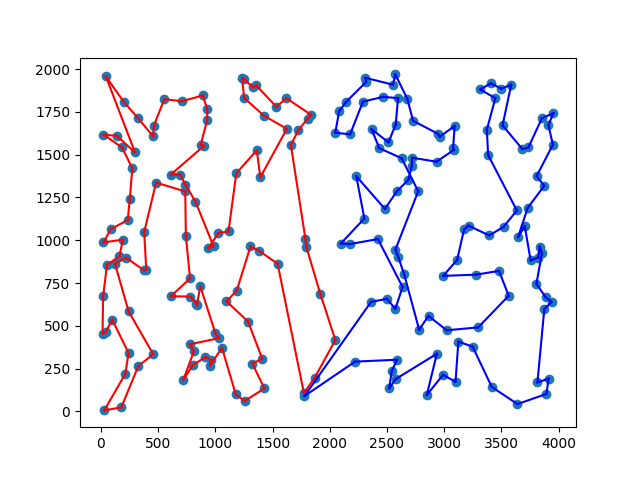
\includegraphics{best_paths/greedy_cheapest_insertion_kroA200.tsp.png}
    \caption{Instancja kroA200}
    \label{fig:Greedy-cycle-kroA}
\end{figure}
\begin{figure}[H]
    \centering
    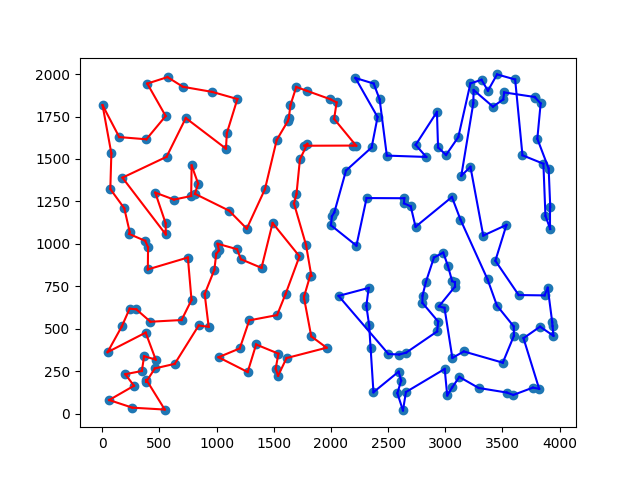
\includegraphics{best_paths/greedy_cheapest_insertion_kroB200.tsp.png}
    \caption{Instancja kroB200}
    \label{fig:Greedy-cycle-kroB}
\end{figure}

\subsection{Algorytm dwużal}\label{subsec:algorytm-dwużal}
Graficzną reprezentację wyników dla algorytmu dwużalu przestawiono na~\ref{fig:Two-regret-kroA} oraz ~\ref{fig:Two-regret-kroB}.

\begin{figure}[H]
    \centering
    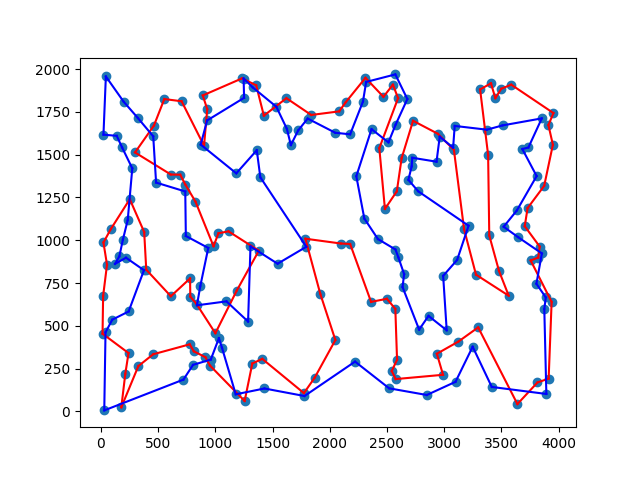
\includegraphics{best_paths/two_regret_kroA200.tsp.png}
    \caption{Instancja kroA200}
    \label{fig:Two-regret-kroA}
\end{figure}
\begin{figure}[H]
    \centering
    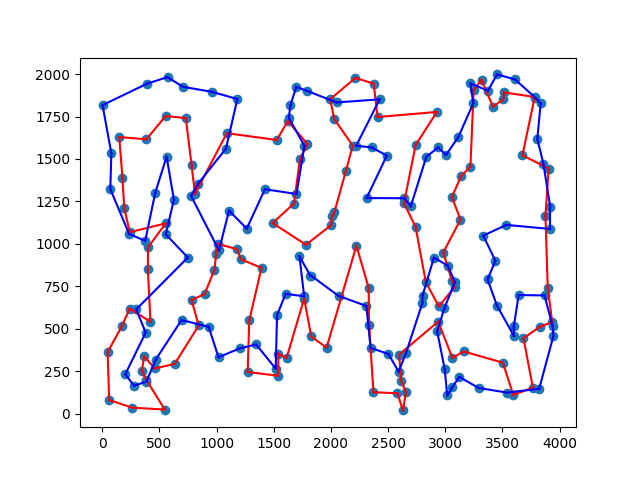
\includegraphics{best_paths/two_regret_kroB200.tsp.png}
    \caption{Instancja kroB200}
    \label{fig:Two-regret-kroB}
\end{figure}

\subsection{Algorytm dwużal ważony}\label{subsec:algorytm-dwużal-ważony}
Graficzną reprezentację wyników dla algorytmu dwużalu ważonego przestawiono na~\ref{fig:Two-regret-weighted-kroA} oraz~\ref{fig:Two-regret-weighted-kroB}.

\begin{figure}[H]
    \centering
    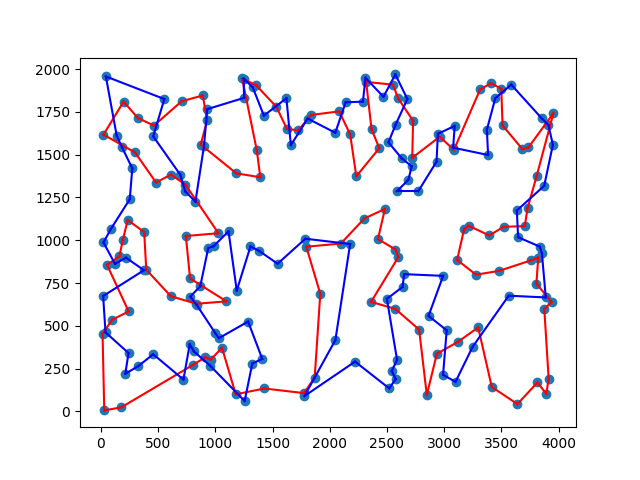
\includegraphics{best_paths/weighted_two_regret_kroA200.tsp.png}
    \caption{Instancja kroA200}
    \label{fig:Two-regret-weighted-kroA}
\end{figure}
\begin{figure}[H]
    \centering
    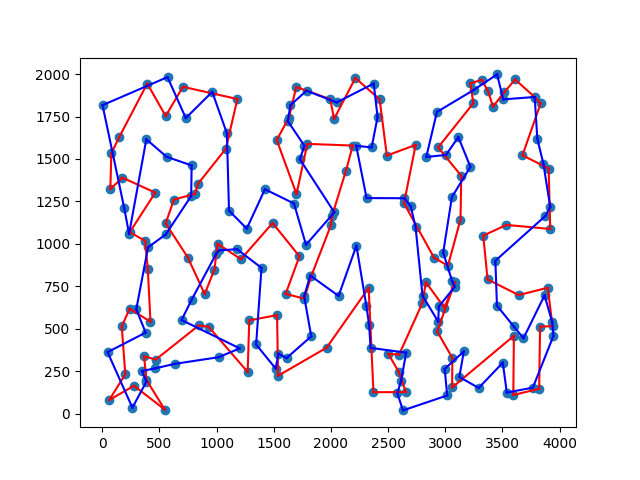
\includegraphics{best_paths/weighted_two_regret_kroB200.tsp.png}
    \caption{Instancja kroB200}
    \label{fig:Two-regret-weighted-kroB}
\end{figure}

\subsection{Algorytm własny}\label{subsec:algorytm-wlasny}
Graficzną reprezentację wyników dla naszego algorytmu przestawiono na~\ref{fig:Our-kroA} oraz~\ref{fig:Our-kroB}.

\begin{figure}[H]
    \centering
    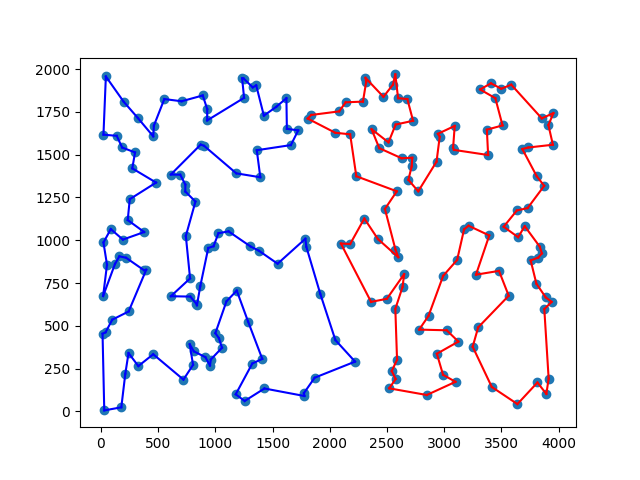
\includegraphics{best_paths/split_paths_regret_TSP_kroA200.tsp.png}
    \caption{Instancja kroA200}
    \label{fig:Our-kroA}
\end{figure}
\begin{figure}[H]
    \centering
    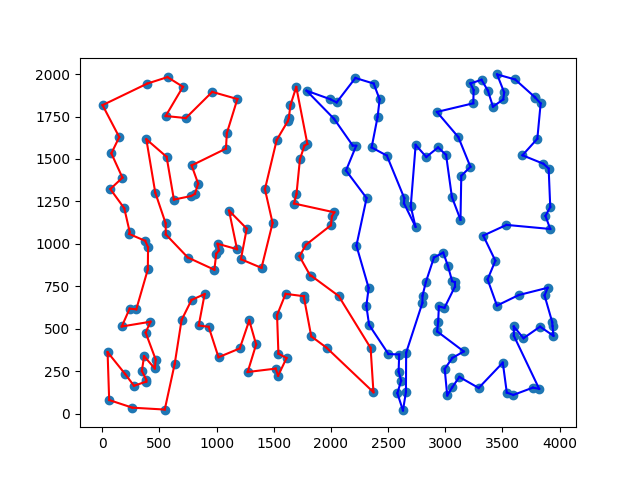
\includegraphics{best_paths/split_paths_regret_TSP_kroB200.tsp.png}
    \caption{Instancja kroB200}
    \label{fig:Our-kroB}
\end{figure}

\section{Porównanie algorytmów}\label{sec:porównanie-algorytmów}
\begin{table}[H]
    \centering
    \begin{tabular}{|c||c|c|c||c|c|c|}
        \hline
        Algorytm & \multicolumn{3}{c||}{KroA200.tsp} & \multicolumn{3}{c|}{KroB200.tsp} \\
        \cline{2-4} \cline{5-7}
        & Min & Średnia & Max & Min & Średnia & Max   \\
        \hline
        Nearest Neighbor Greedy & 36851.00 & 42103.95 & 48120.00 & 38444.00 & 42340.77 & 45918.00 \\
        \hline
        Cycle Extension Greedy & 35396.00 & 38319.41 & 39990.00 & 35295.00 & 38455.17 & 40028.00 \\
        \hline
        Two regret & 42468.00 & 44647.83 & 46393.00 & 41176.00 & 43544.62 & 44972.00 \\
        \hline
        Weighted Two regret & 49770.00 & 51252.74 & 52662.00 & 48911.00 & 50172.06 & 52187.00 \\
        \hline
        Split + Two regret & 30293.00 & 33044.22 & 36854.00 & 31218.00 & 33317.82 & 36913.00 \\
        \hline
    \end{tabular}
    \caption{Wyniki eksperymentu obliczeniowego}
    \label{tab:wyniki-eksperymentu}
\end{table}

\section{Wnioski}\label{sec:wnioski}

Obydwa podejścia wykorzystujące heurystyki związane z żalem przyniosły znacznie gorsze skutki niż znacznie prostsze od nich podejścia zachłanne,
takie jak dodawanie najbliższego sąsiada do obecnie budowanego cyklu, czy rozbudowa cyklu o najtańszy węzeł.
Z graficznej reprezentacji można wywnioskować potencjalne powody dlaczego tak się dzieje - przede wszystkim, obydwa algorytmy oparte na dwu-żalu skonstruowały rozłączne cykle które często się przecinały,
podczas gdy algorytm rozbudowy cyklu o najtańszy wierzchołek budował cykle które ``nie wchodziły sobie w drogę''.
Dzieje się tak przede wszystkim ze względu na to, że algorytm nie bierze pod uwagę tego że budujemy dwa rozłączne cykle i ``nie musi żałować'' połowy wierzchołków które sprawdza.
W tym momencie pojawia się kilka pomysłów na rozwiązanie tego problemu! \\
Po pierwsze, można by jakoś podzielić zbiór wierzchołków na dwa równe podzbiory i wtedy wywołać na nich osobno algorytm oparty na żalu.
Można pokusić sie np.\ o wykorzystanie algorytmu k-means, lub dla naszego problemu zmodyfikować go aby tworzył zbalansowane klastry.
Po drugie, można zmodyfikować algorytm wykorzystujący dwużal o to, aby dla każdego wierzchołka wyliczany był żal dołączenia go do pierwszego cyklu, jak i do drugiego jednocześnie,
a następnie branie go pod uwagę tylko dla cyklu który ma mniejszy żal dołączenia go.
To niestety znów powoduje problemy z balansowaniem długości obu cykli i ma tendencję do tworzenia jednego cyklu obejmującego znaczną większośc wierzchołków
(>90\% oraz drugiego, drobnego na kilka wierzchołków lub czasem obejmującego tylko wierzchołek startowy).
Próby wymuszenia balansowania cykli niestety prowadziły do wyników bardzo zbliżonych do podstawowych algorytmów wykorzystujących dwużal oraz dwużal ważony.
Znacznie lepiej jednak zadziałał algorytm z pierwszego pomysłu, mimo że nie wykorzystaliśmy w nim k-means do podziału zbioru wierzchołków a zachłanną metodę znajdywania n/2 najbliższych do wierzchołka startowego.
Główny powód dla którego zdecydowaliśmy się na taką metodę podziału, to aby zostać w duchu pozostałych algorytmów i porównać ze sobą metody zachłanne.

\section{Link do repozytorium}\label{sec:link-do-repo}
Kod źródłowy w repozytorium GitHub dostępny pod linkiem: \\
\href{https://github.com/KotZPolibudy/PUT_IMO/tree/main/TSP_heuristic}{Repozytorium TSP Heuristics}.

\end{document}
